\documentclass[t,ucs,12pt,xcolor=dvipsnames]{beamer}
\usepackage{graphicx}
\usepackage{hyperref}
\usepackage{float}
\graphicspath{ {/Users/jiayuan/Documents/MA881/markdown/} }

\title{Boston Home Price Index Analysis}
\author{Jiayuan Shi}
\date{\today}

\usepackage{Sweave}
\begin{document}
\Sconcordance{concordance:beamer.homeprice.tex:beamer.homeprice.Rnw:%
1 10 1 1 0 17 1 1 7 1 2 46 1}




\setkeys{Gin}{width=0.6\textwidth}

\maketitle

In 2008, the US ecomony faces the most dangerous financial crisis, which expanded to Asia, Europe and other places around the world. The stock market was plummeted nearly 0.3; credit market was ceased to function; Lehman Brothers went bankcrupt overnight;Prices of houses was dropping and people had low faith to the economy.\

In the first chapter of Nate Silver's \textit{The Signal and the Noise}, we were told housing prices continued their inexorable decline, falling a lot during 2008. Now we are looking into the historical home price index for Boston. We want to compare the changes of housing price in U.S.A from 2000 to 2015, in order to see if there is a larger falling in 2008.\

This home price index seeks to measure the value of residential real estate in the City of Boston from year 2000 to 2015, on a monthly basis. For more details, please go to the following website: \url{http://us.spindices.com/indices/real-estate/sp-case-shiller-20-city-composite-home-price-index}. 

First, we make a graph to show housing price monthly change in Boston.
\begin{figure}[H]
 \begin{center}
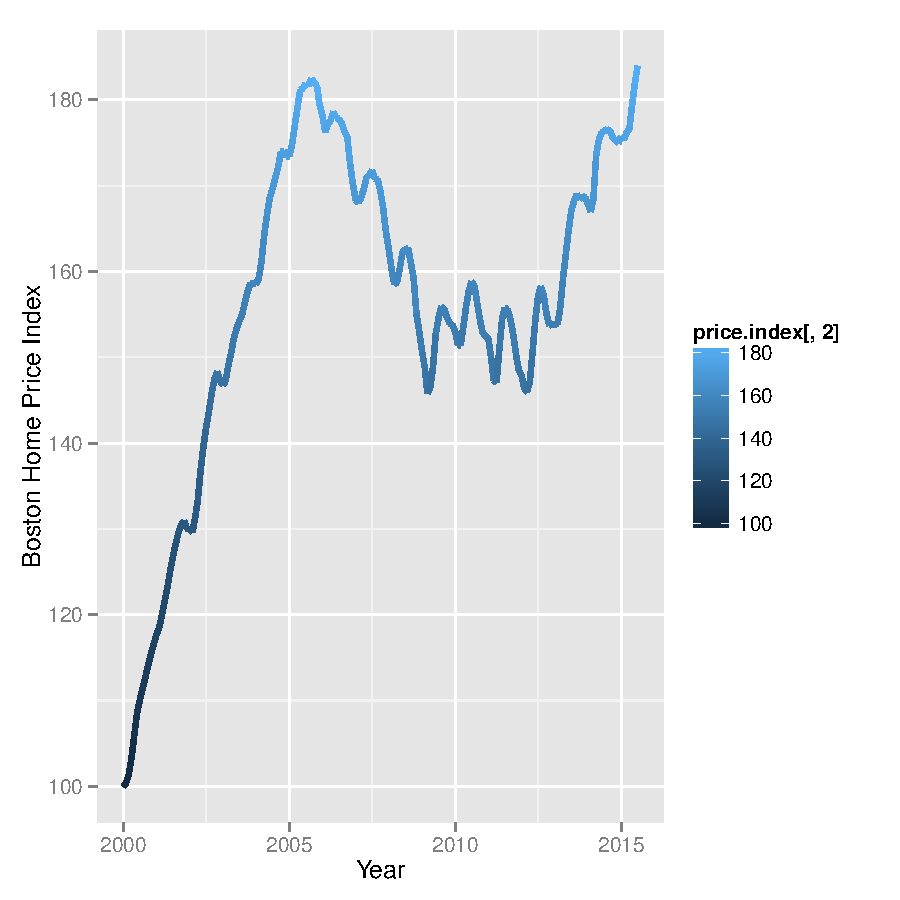
\includegraphics{fig--001}
 \caption{Housing Price Change from 2000 to 2015}
 \end{center}
\end{figure}
In the gragh, we find that the housing price of Boston is firstly growing-up then falling-down, and growing up again. The housing price increases a lot from 2000, but start to decrease from 2005, and increase a lot again from 2011.\\

There is a graph from the S\&P website about the home price index for Boston during 1985 and 2015, which we can also see the same "up-down-up" pattern from 2000 to 2015.

\begin{figure}[H]
  \centering
  \includegraphics[width=\linewidth]{Housing.png}
  \caption{Housing Price Change from 1985 to 2015}
\end{figure}

The yearly mean housing price of Boston is presented in table. And we calculate the year-over-year housing index change. 
\begin{table}[H]
\centering
\caption{Housing Price Change from 2000 to 2015}
\label{my-label}
\begin{tabular}{lll}
Year & Boston   & Change  \\
2000 & 108.2792 &         \\
2001 & 125.17   & 15.60\% \\
2002 & 139.5625 & 11.50\% \\
2003 & 153.2692 & 9.82\%  \\
2004 & 167.7067 & 9.42\%  \\
2005 & 179.6558 & 7.12\%  \\
2006 & 176.3108 & -1.86\% \\
2007 & 169.2792 & -3.99\% \\
2008 & 159.6875 & -5.67\% \\
2009 & 151.8183 & -4.93\% \\
2010 & 154.6858 & 1.89\%  \\
2011 & 151.5858 & -2.00\% \\
2012 & 152.2992 & 0.47\%  \\
2013 & 163.2817 & 7.21\%  \\
2014 & 173.6267 & 6.34\%  \\
2015 & 178.4414 &        
\end{tabular}
\end{table}

From the chart, we can also see that the housing price of Boston increases a lot from 2000, but start to decrease from 2005, and increase a lot again from 2011. From 2007 to 2009, the housing price a larger decrease, which is -5.67\% and -4.93\%.

The equation about how to calculate the year-over-year housing index change is shown below.
\[f\left ( x \right )= \frac{y_{t}-y_{t-1}}{y_{t-1}} * 100\]

To sum up, the housing price of Boston is firstly growing-up then falling-down, and growing up again. The housing price increases a lot from 2000, but start to decrease from 2005, and increase a lot again from 2011. From 2007 to 2009, the housing price a larger decrease, which is -5.67\% and -4.93\%. The conclusion is consistent with Nate Silver's book \textit{The Signal and the Noise}, in which we were told housing prices continued their inexorable decline, falling a lot during 2008.  

\end{document}
